\section{Results and Discussion}
The Simulink-aided implemented design can be observed in Fig~\ref{fig:heat_system_diagram}. The output of the system, denoted as $x_{k}$, is connected to a display for real-time visualization of the parameter estimation ($\phi$ and $\Gamma$). Additionally, the input function (sum of unit step functions), the ambient temperature readings, and the prediction of the system ($x_{k}$) are connected for waveform analysis and verification.

\begin{figure}[H]
\centering
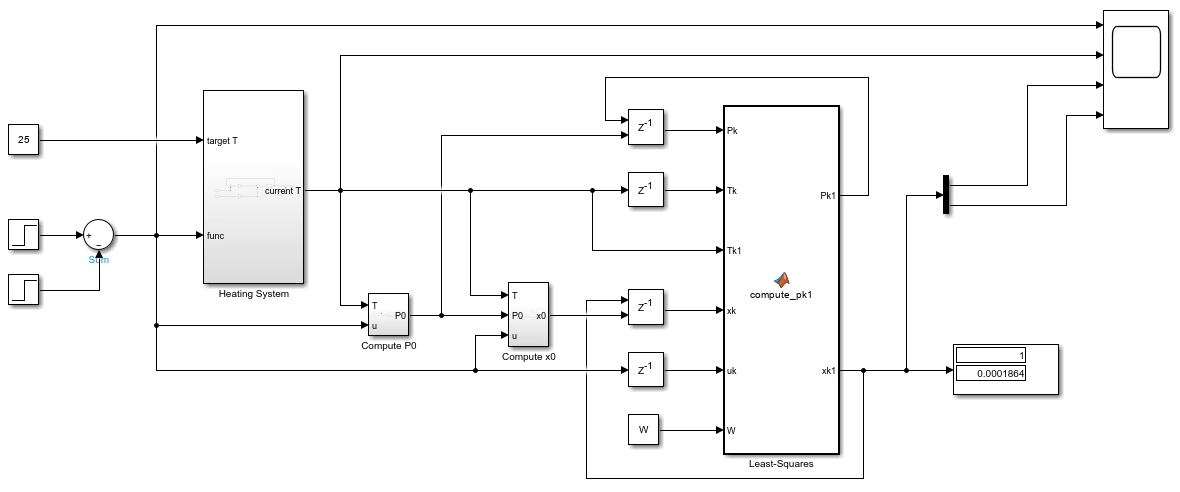
\includegraphics[width=1\linewidth]{figures/simulink_system.png}
\caption{}
~\label{fig:simulink_system}
\end{figure}

The initial scenario involves a solitary measurement of the temperature. Fig~\ref{fig:simulink_plot} shows the corresponding waveforms. The first column illustrates the input function alongside the recorded temperature. Meanwhile, the second column depicts the estimation of the filter.

\begin{figure}[H]
\centering
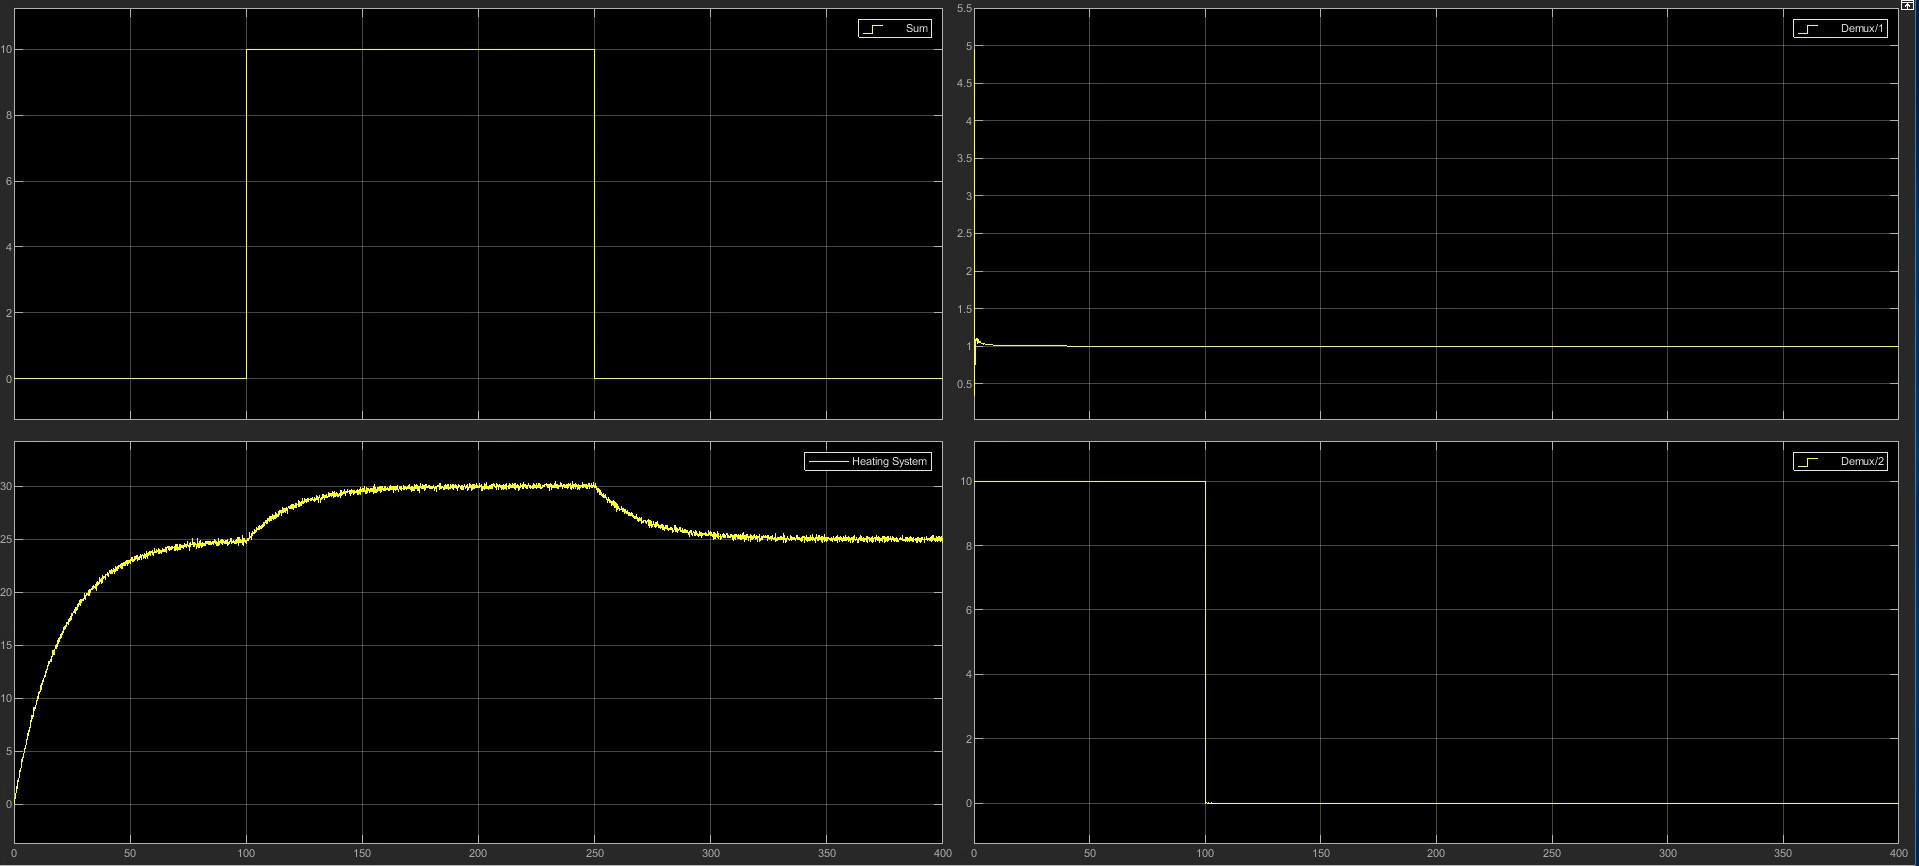
\includegraphics[width=1\linewidth]{figures/simulink_plot.png}
\caption{In the first column are the input function and measured temperature. In the second column are the filter estimations}
~\label{fig:simulink_plot}
\end{figure}

Fig~\ref{fig:simulink_params} presents the estimation of the parameters. The system estimates $\phi = 1$ and $\Gamma = 0.0001864$, reflecting a relative error of $\phi_{error} = 0.5\%$ and $\Gamma_{error} = 92\%$. Despite the relatively high error in $\Gamma$, the system's overall accuracy for a single sample remains commendable.

\begin{figure}[H]
\centering
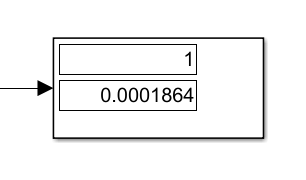
\includegraphics[width=0.55\linewidth]{figures/simulink_params.png}
\caption{$\phi$ and $\Gamma$ estimation using just one sample of the temperature}
~\label{fig:simulink_params}
\end{figure}

In the second scenario, leveraging multiple temperature samples significantly enhances the system's estimation capabilities. Fig~\ref{fig:simulink_params_gen} illustrates the estimation of the parameters based on this expanded dataset. In this scenario, the system estimates $\phi = 0.9975$ and $\Gamma = 0.002558$ resulting in a relative error of $\phi_{error} = 3\%$ and $\Gamma_{error} = 9\%$. These findings underscore the system's enhanced accuracy as it benefits from a richer dataset, showcasing its capacity to improve with increased data input.

\begin{figure}[H]
\centering
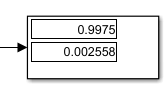
\includegraphics[width=0.4\linewidth]{figures/simulink_params_gen.png}
\caption{$\phi$ and $\Gamma$ estimation using multiple samples of the temperature}
~\label{fig:simulink_params_gen}
\end{figure}
